\documentclass[12pt,a4paper]{article}
\usepackage[margin=2cm]{geometry}
\usepackage{amsmath,amsthm,amssymb}
\usepackage{CJK}
\usepackage{verbatim}
\usepackage{graphicx}

\begin{document}
	\begin{CJK}{UTF8}{bsmi}
		參數設定: 
		\begin{enumerate}
			\item 時間區間 $[0,25]$
			\item 原始細胞膜厚度 $h_0=0.005$
			\item 縮放倍數 $scale$
			\item 時間尺度 $\epsilon$
		\end{enumerate}
		當細胞膜增厚時,給定增厚函數為
		$$h(t)=\frac{h_0(scale+e^{-\frac{t-12.5}{\epsilon}})}{1+e^{-\frac{t-12.5}{\epsilon}}}$$
		\begin{figure}[htbp]
			\centering
			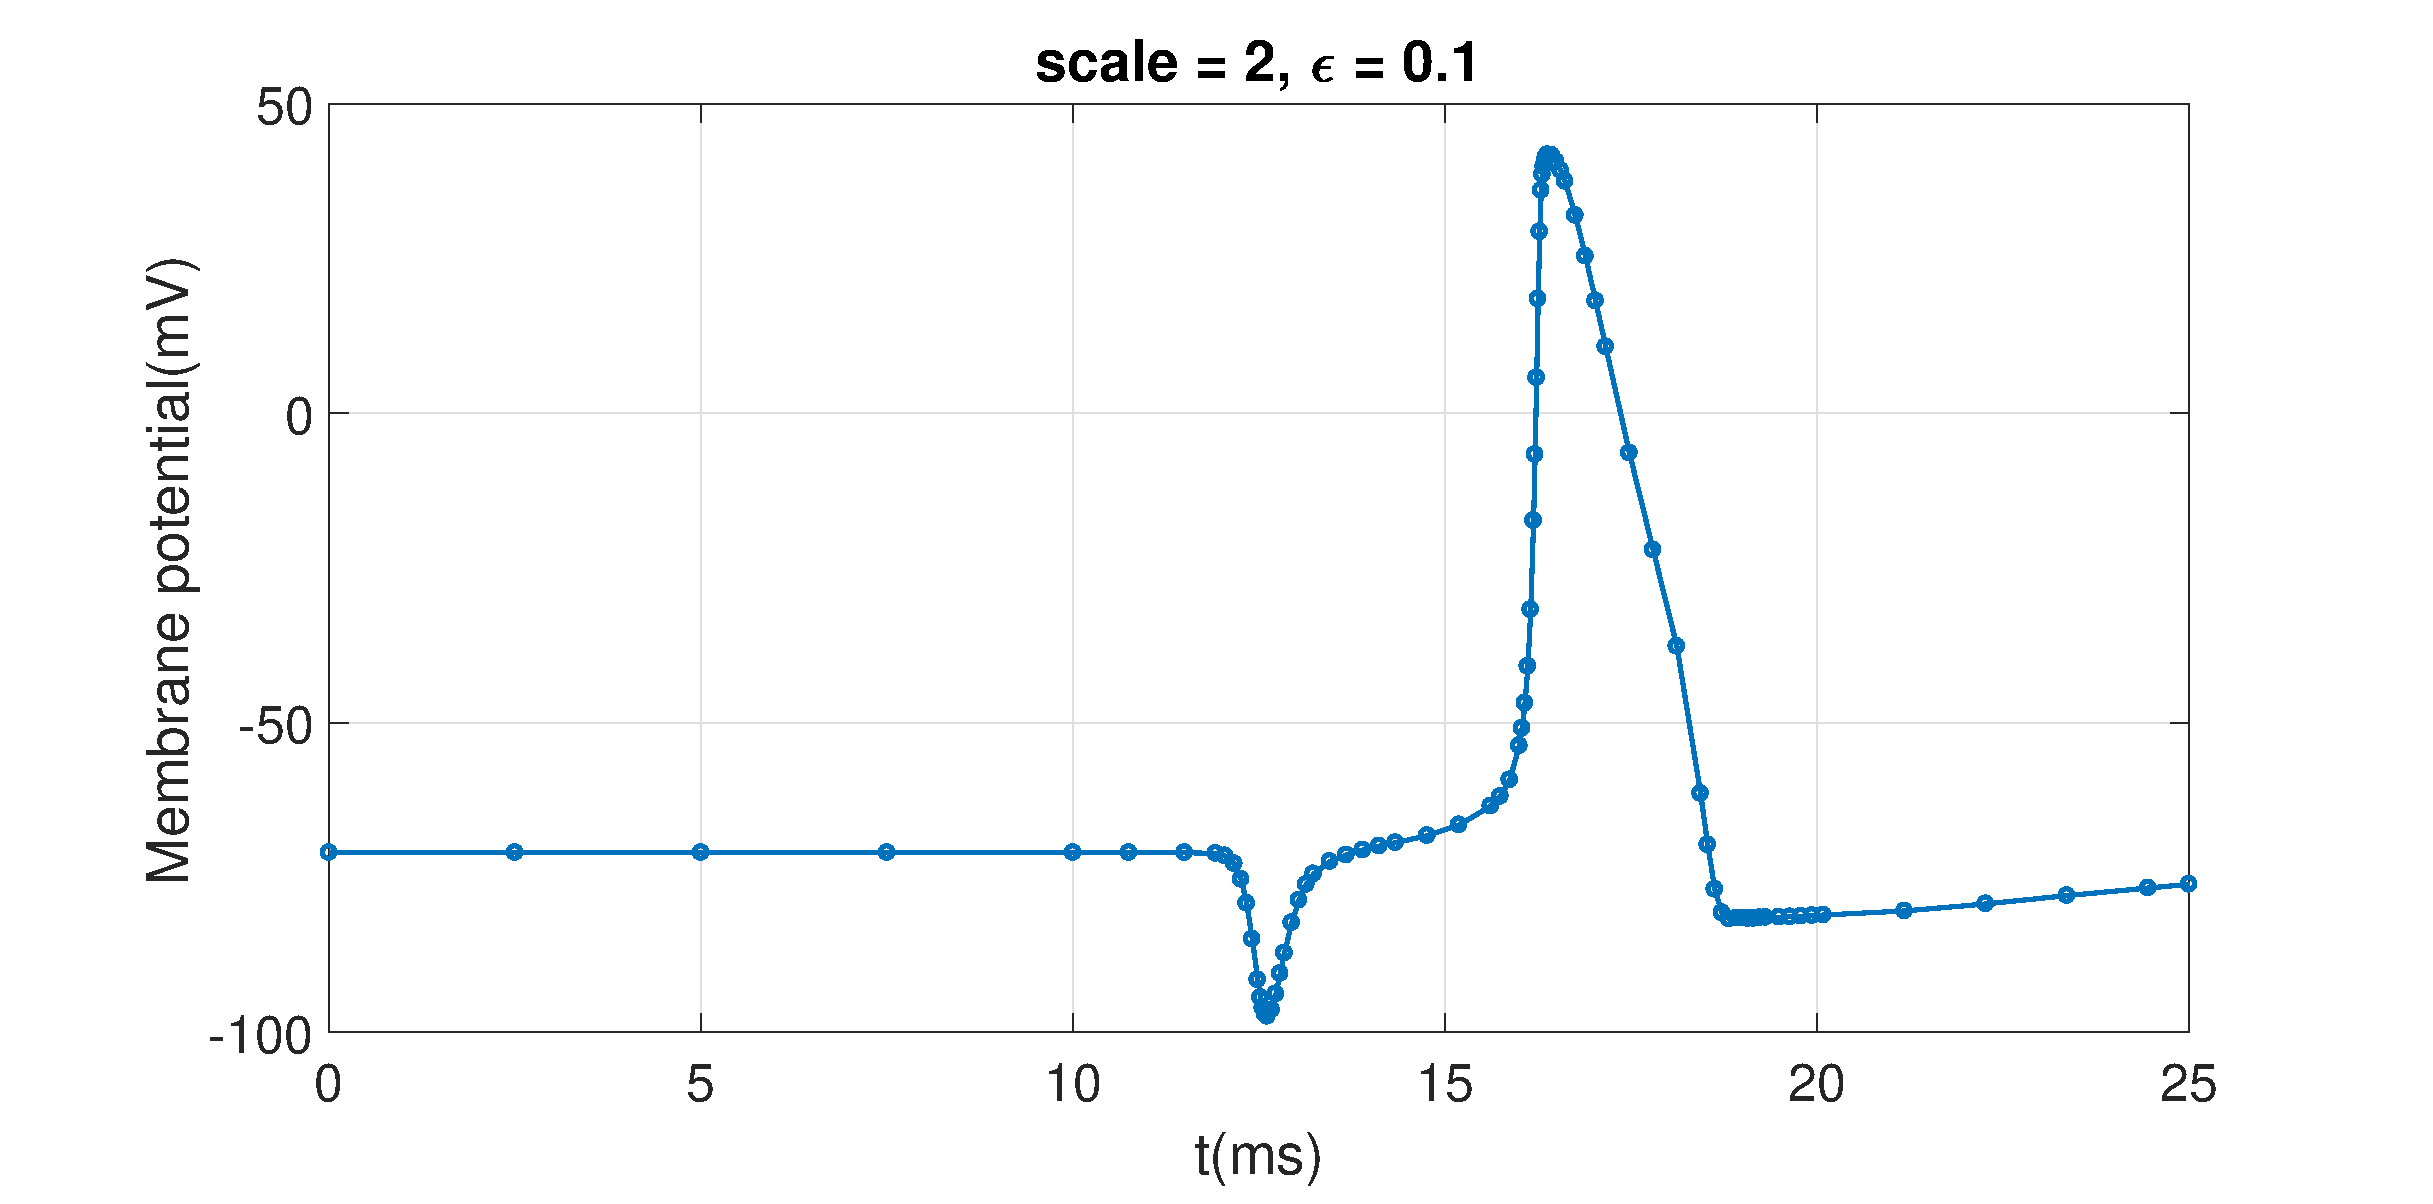
\includegraphics[width = 500pt]{21.eps}
		\end{figure}
		\begin{figure}[htbp]
			\centering
			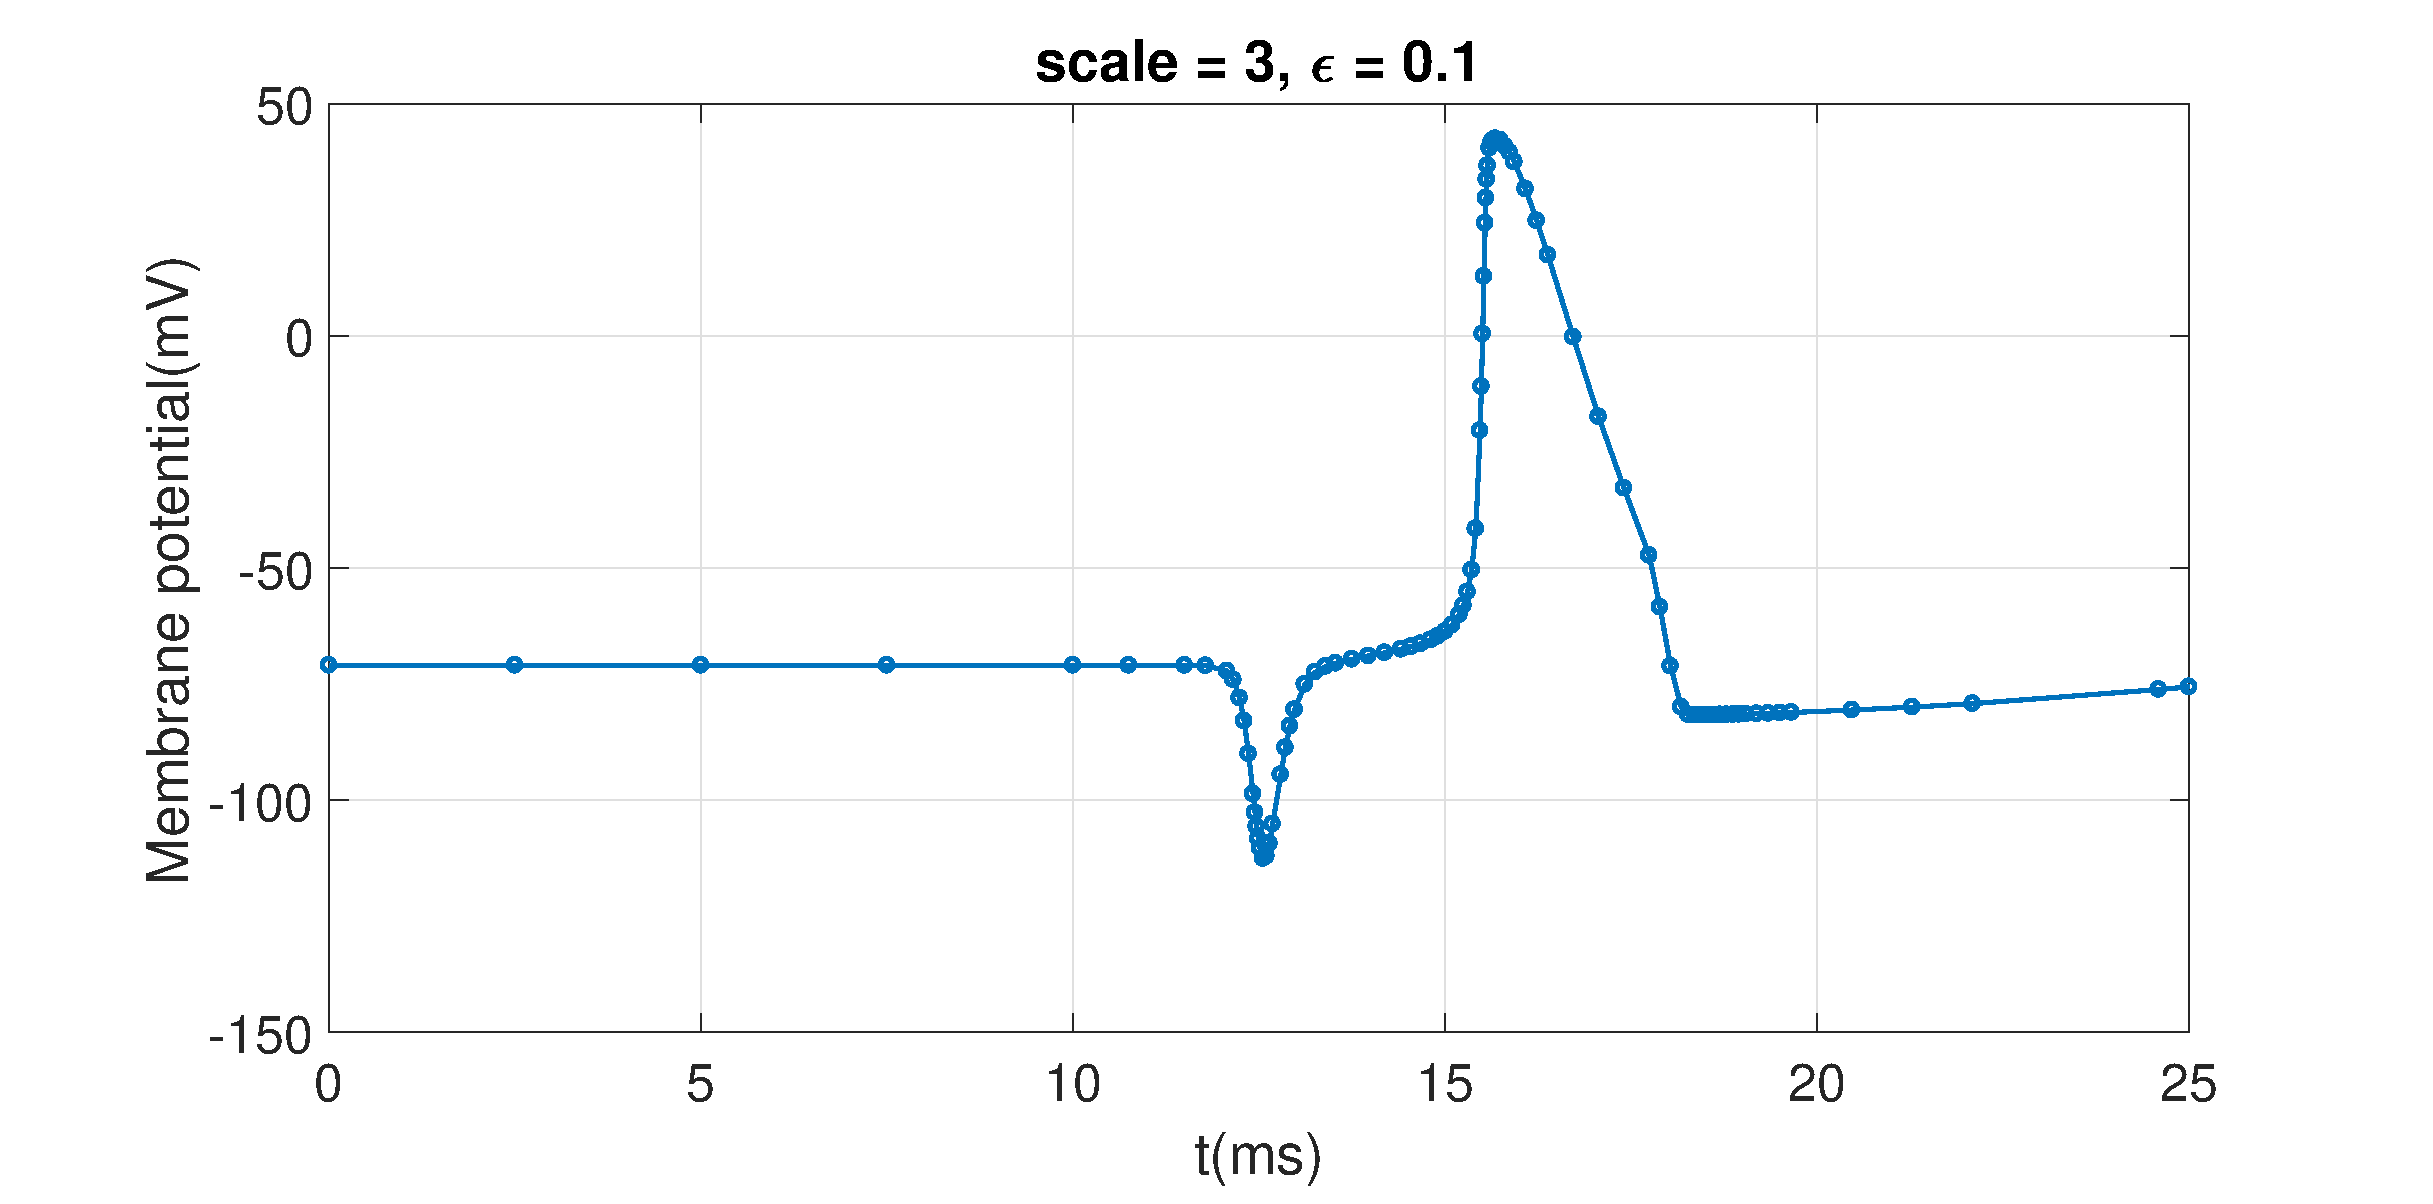
\includegraphics[width = 500pt]{31.eps}
		\end{figure}
		\begin{figure}[htbp]
			\centering
			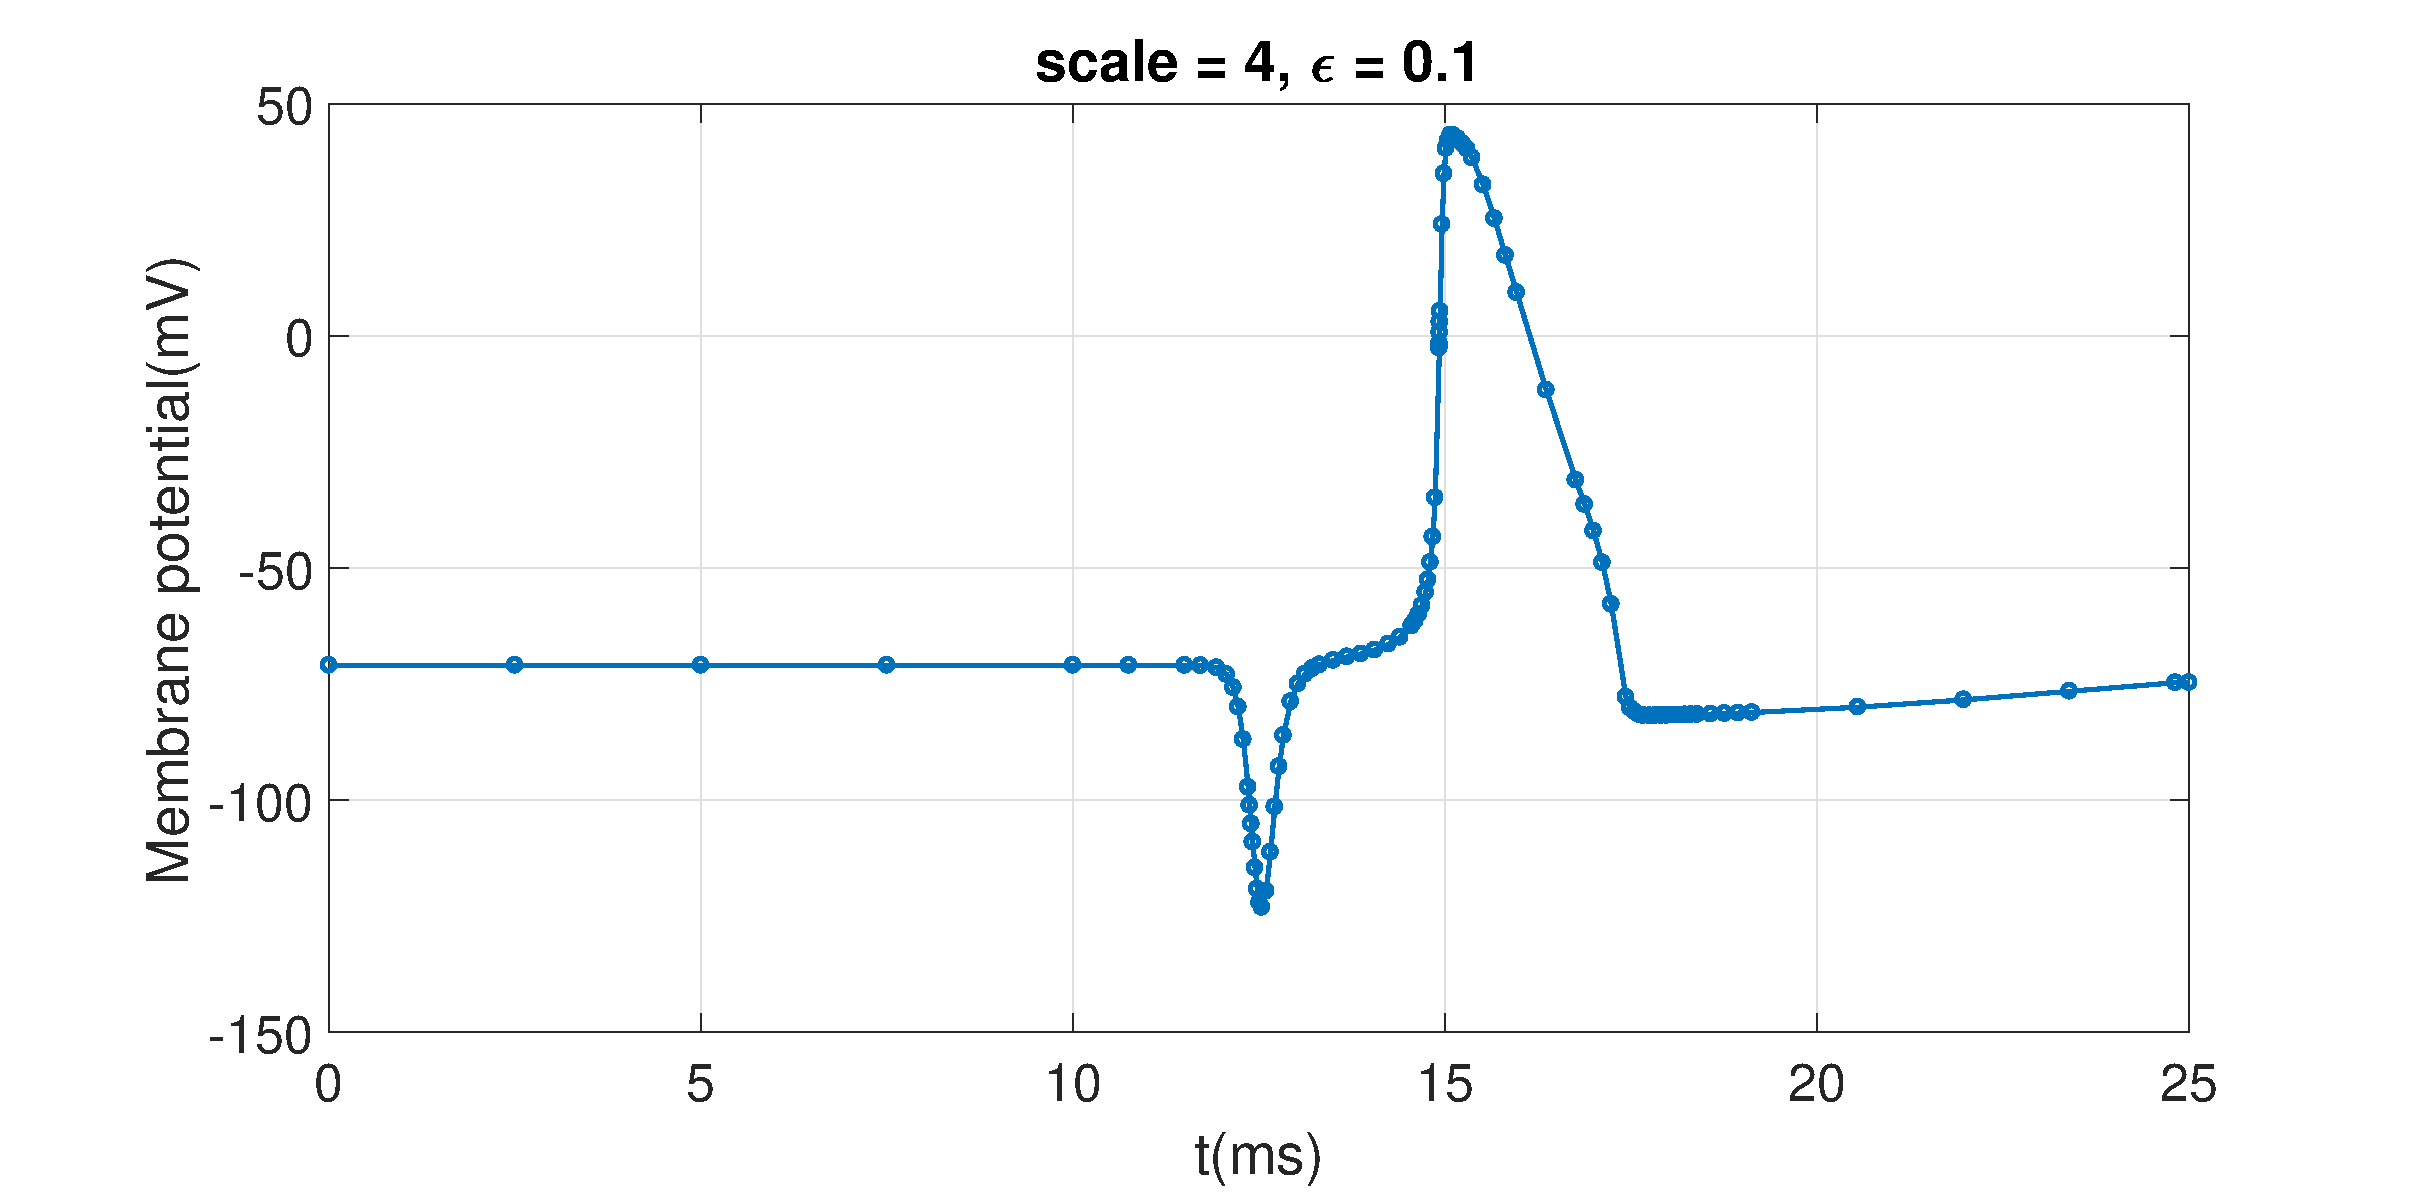
\includegraphics[width = 500pt]{41.eps}
		\end{figure}
		\begin{figure}[htbp]
			\centering
			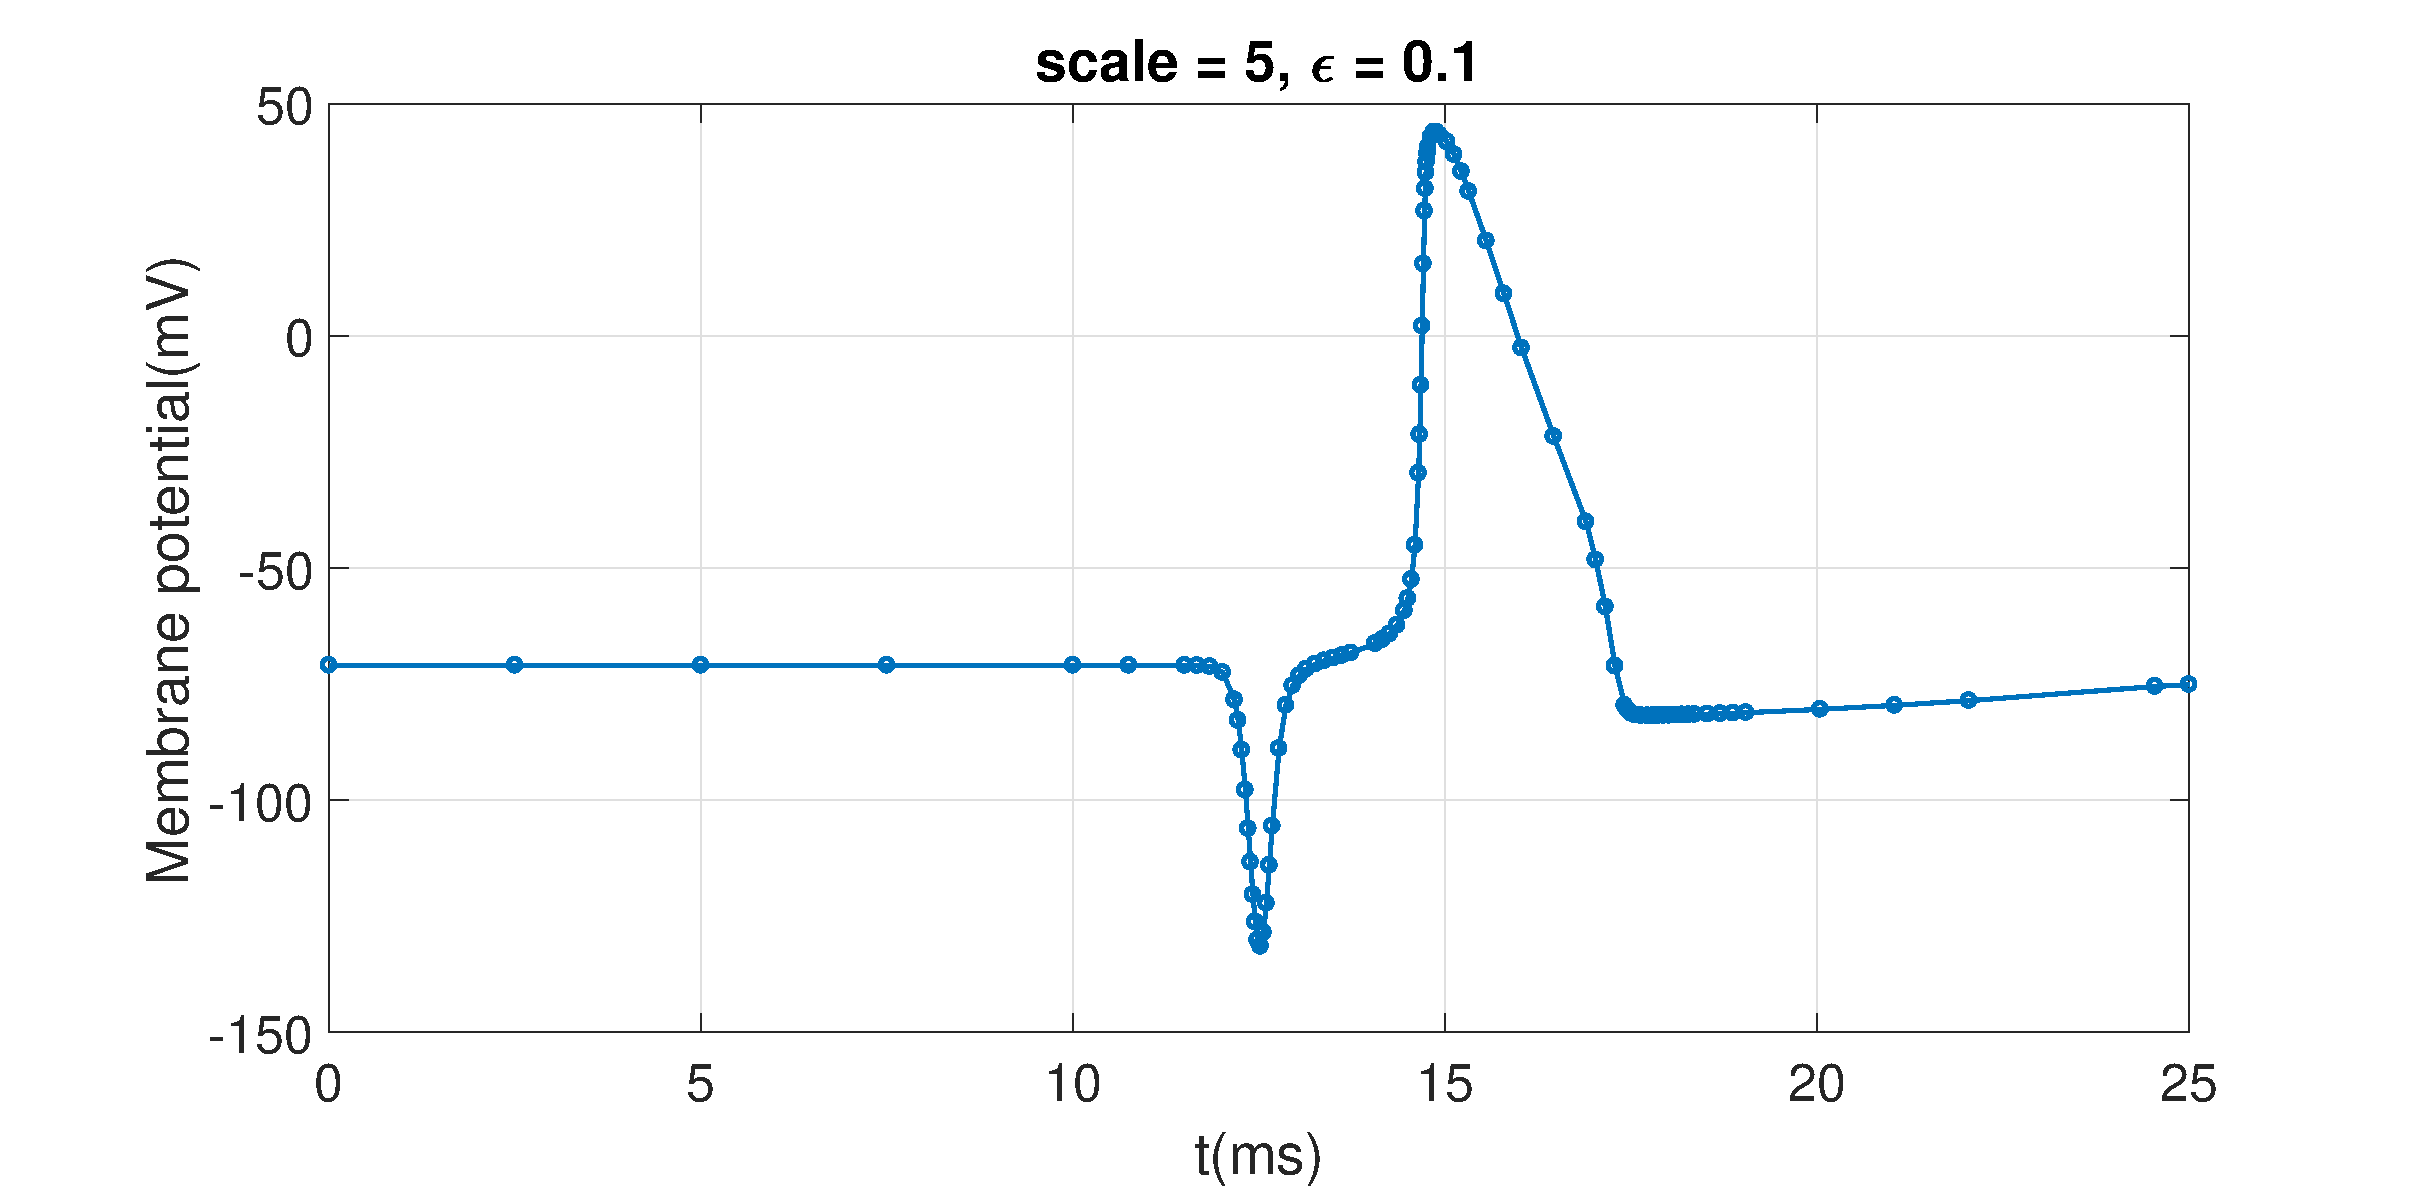
\includegraphics[width = 500pt]{51.eps}
		\end{figure}
		\begin{figure}[htbp]
			\centering
			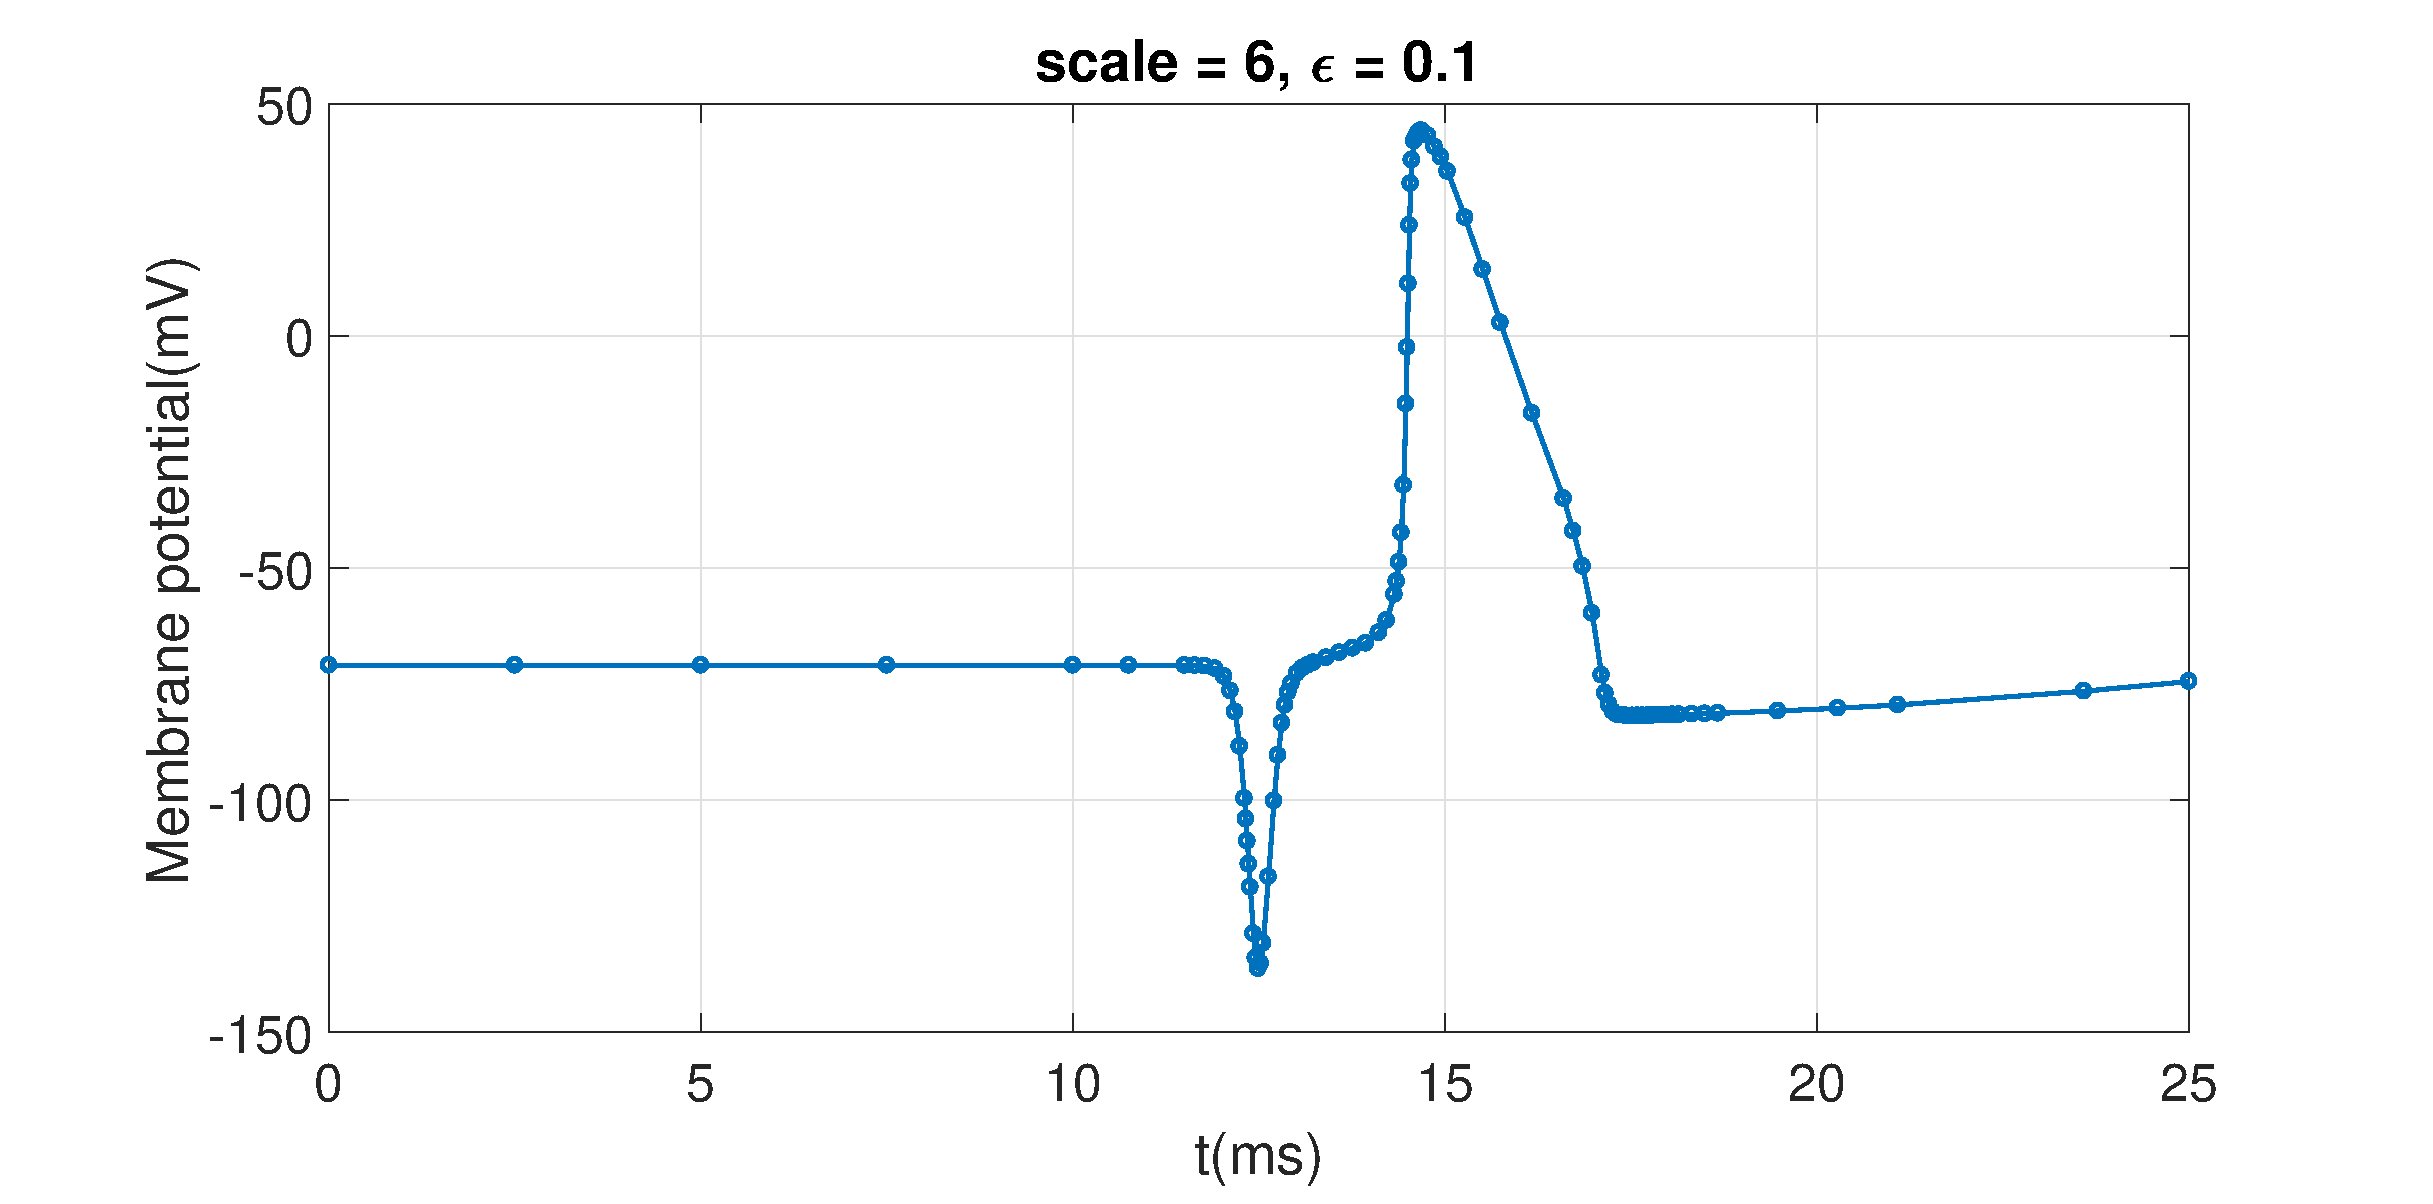
\includegraphics[width = 500pt]{61.eps}
		\end{figure}
	\newpage
	當細胞膜變薄時,給定變薄函數為
	$$h(t)=\frac{h_0(1+scale e^{\frac{t-12.5}{\epsilon}})}{1+e^{\frac{t-12.5}{\epsilon}}}$$
	\begin{figure}[htbp]
		\centering
		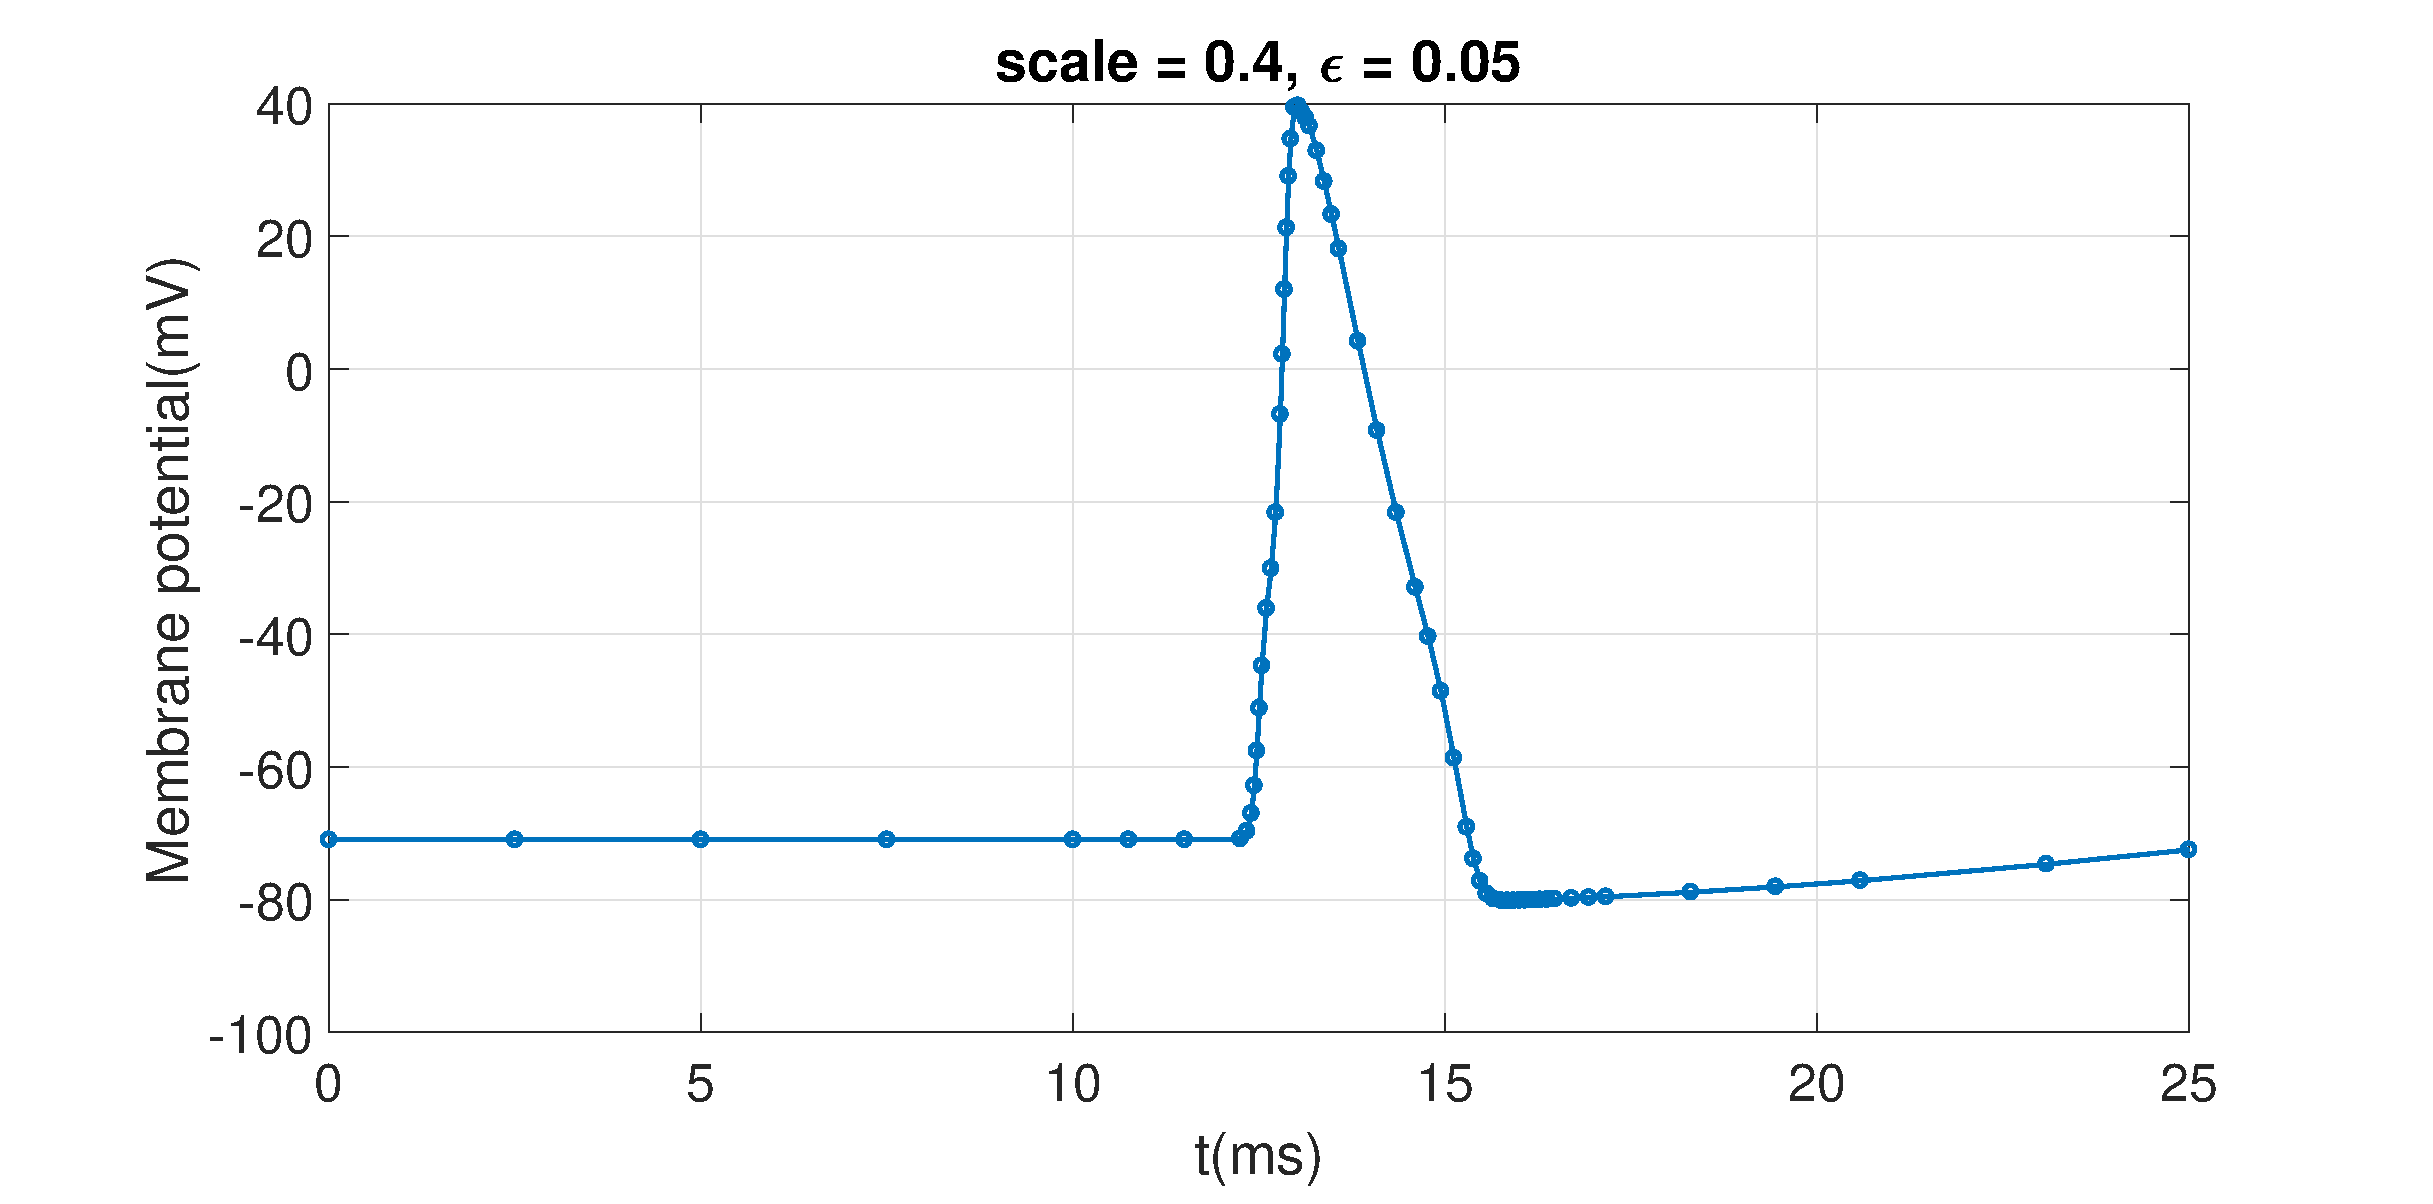
\includegraphics[width = 500pt]{405.eps}
	\end{figure}
	\begin{figure}[htbp]
		\centering
		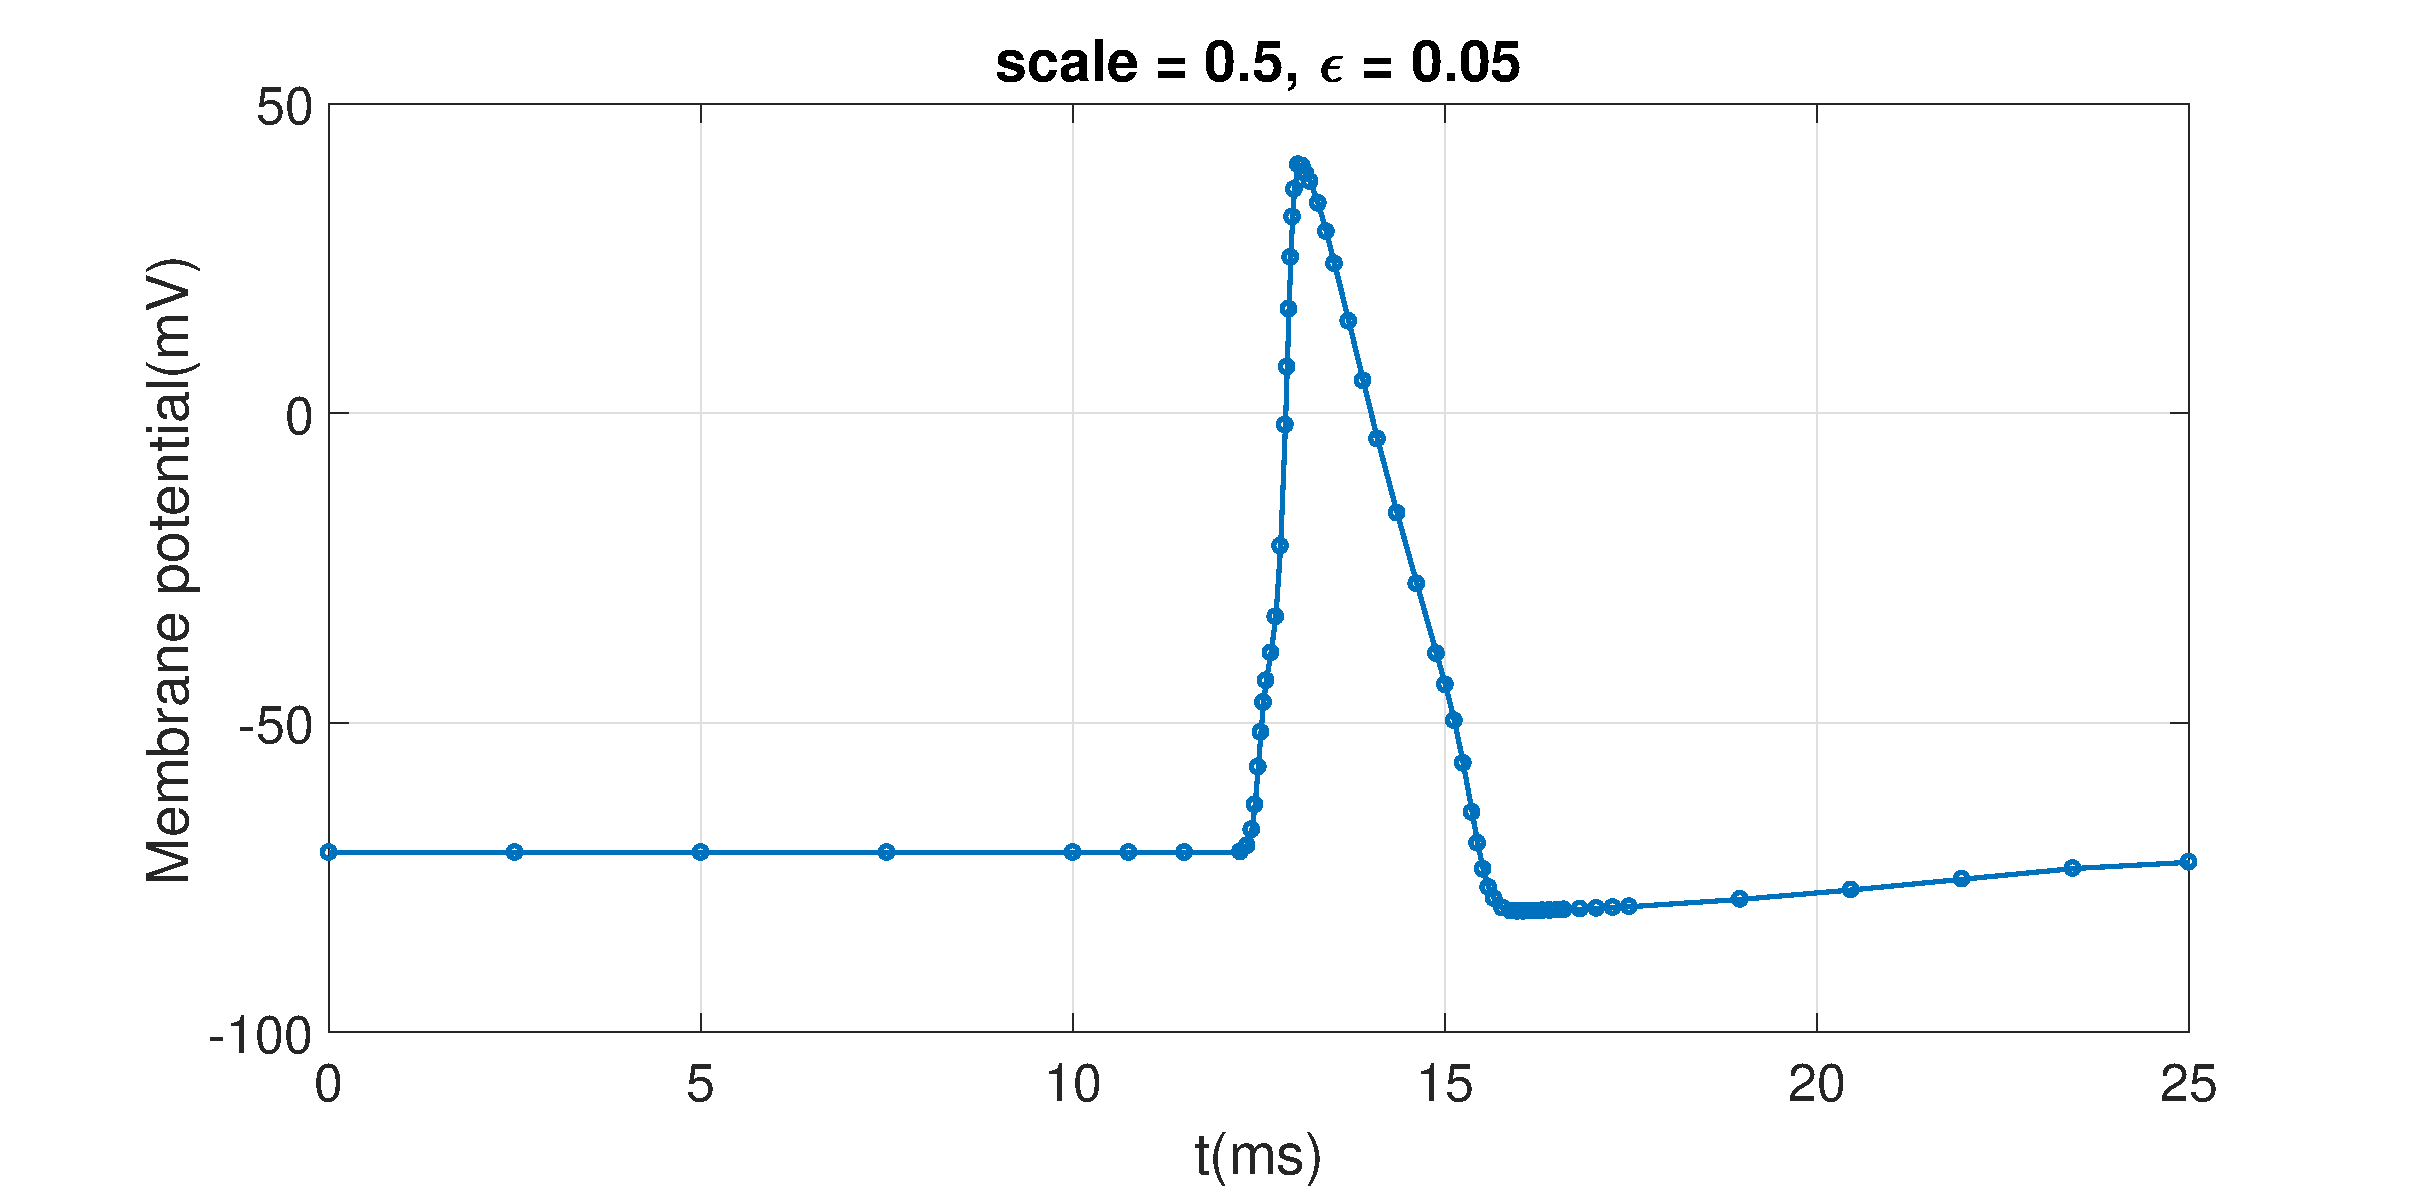
\includegraphics[width = 500pt]{505.eps}
	\end{figure}
	\begin{figure}[htbp]
		\centering
		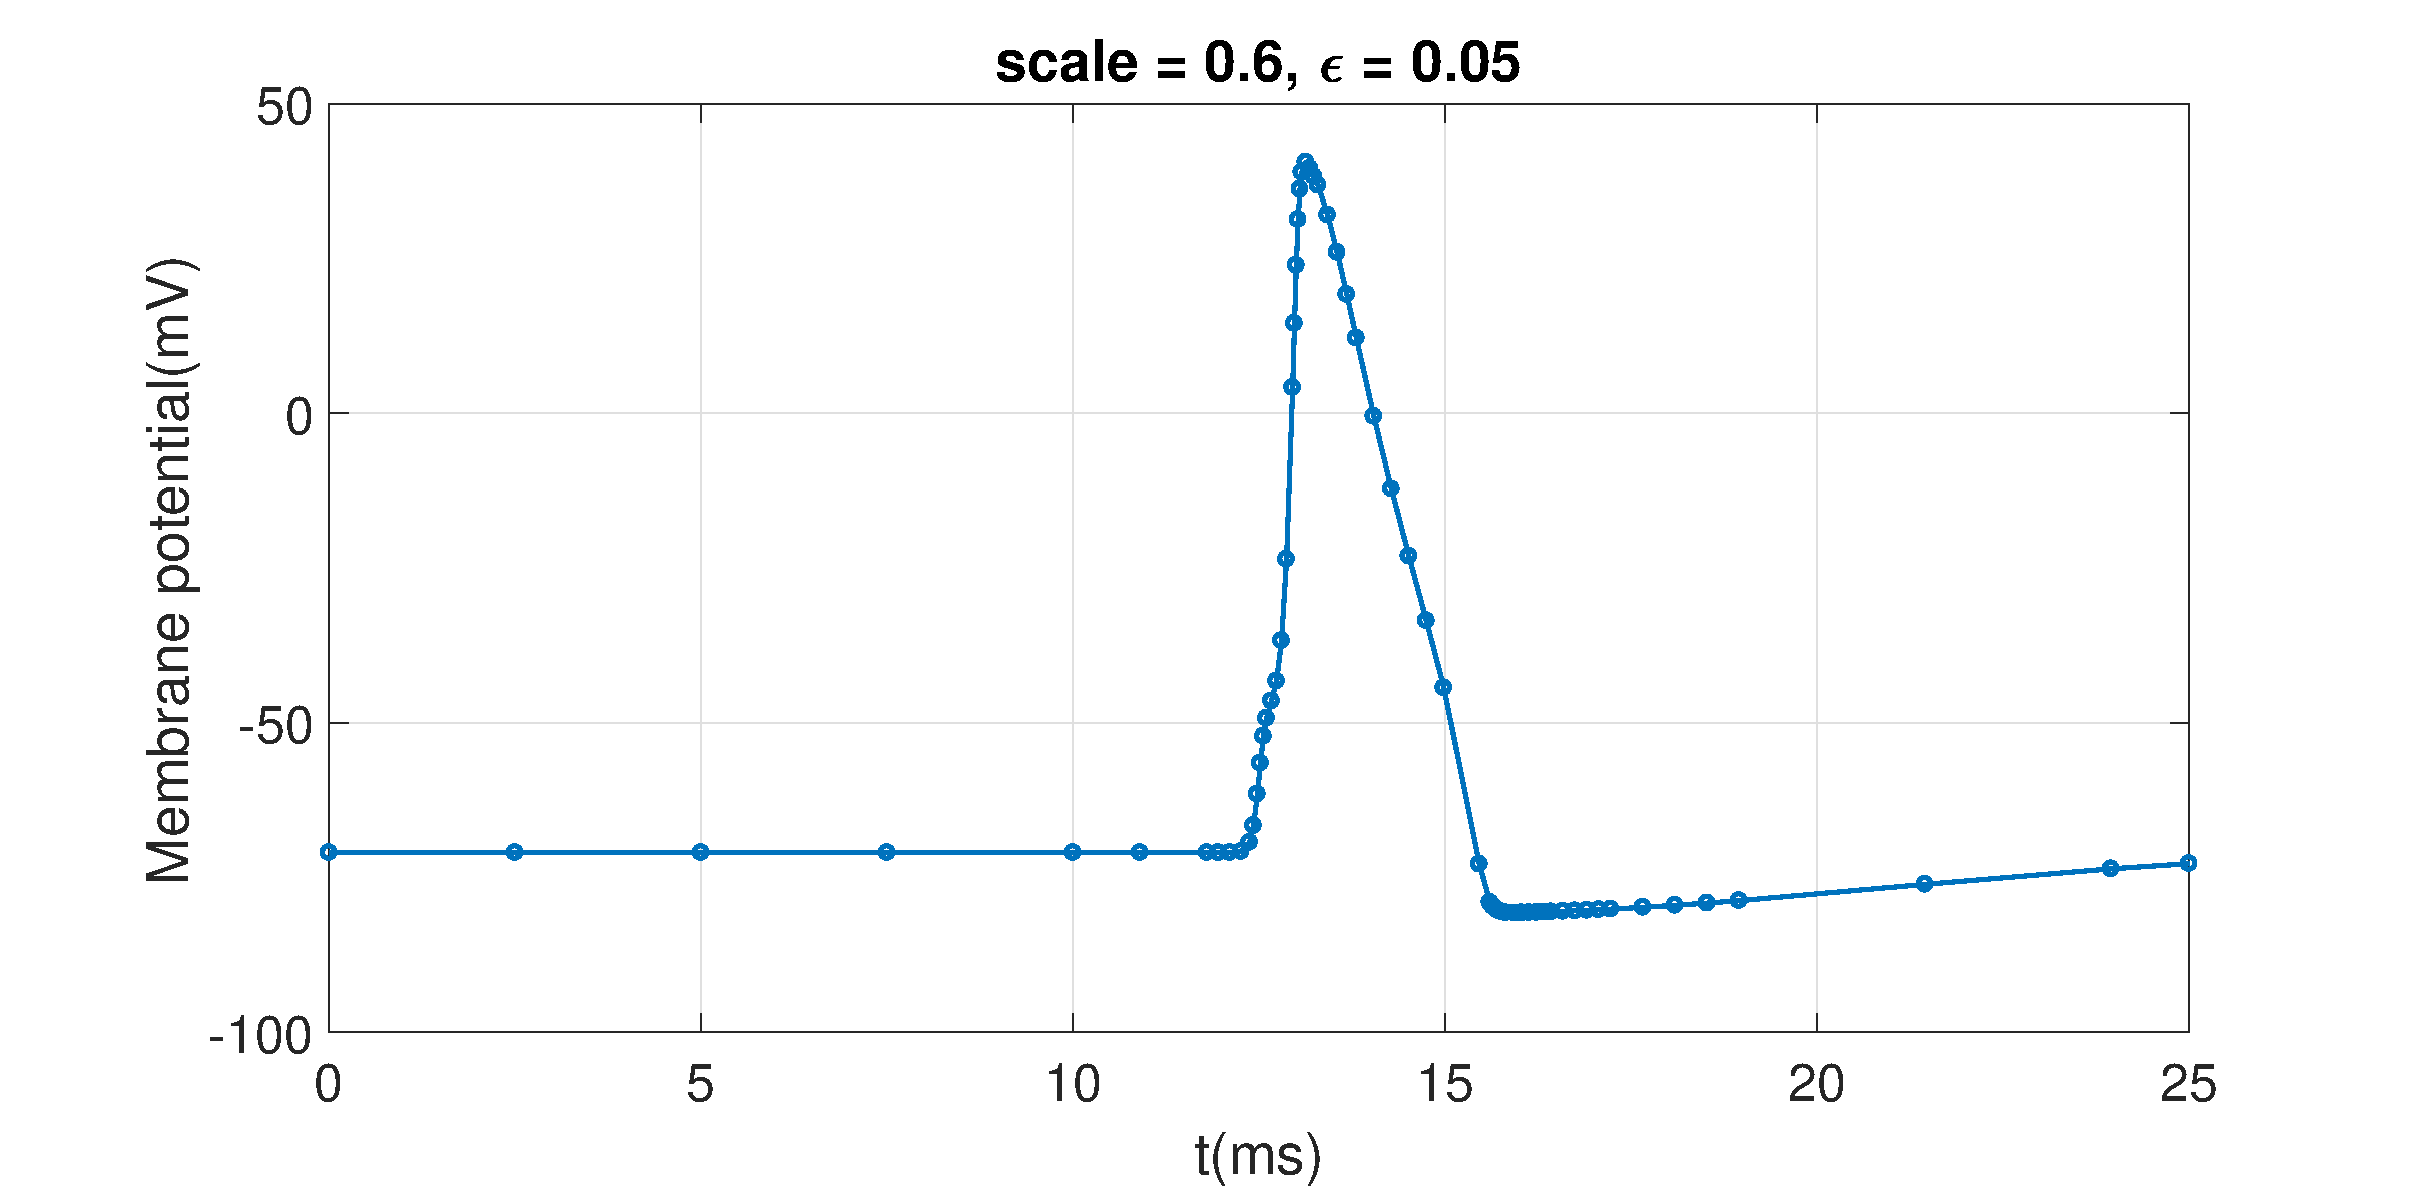
\includegraphics[width = 500pt]{605.eps}
	\end{figure}
	\begin{figure}[htbp]
		\centering
		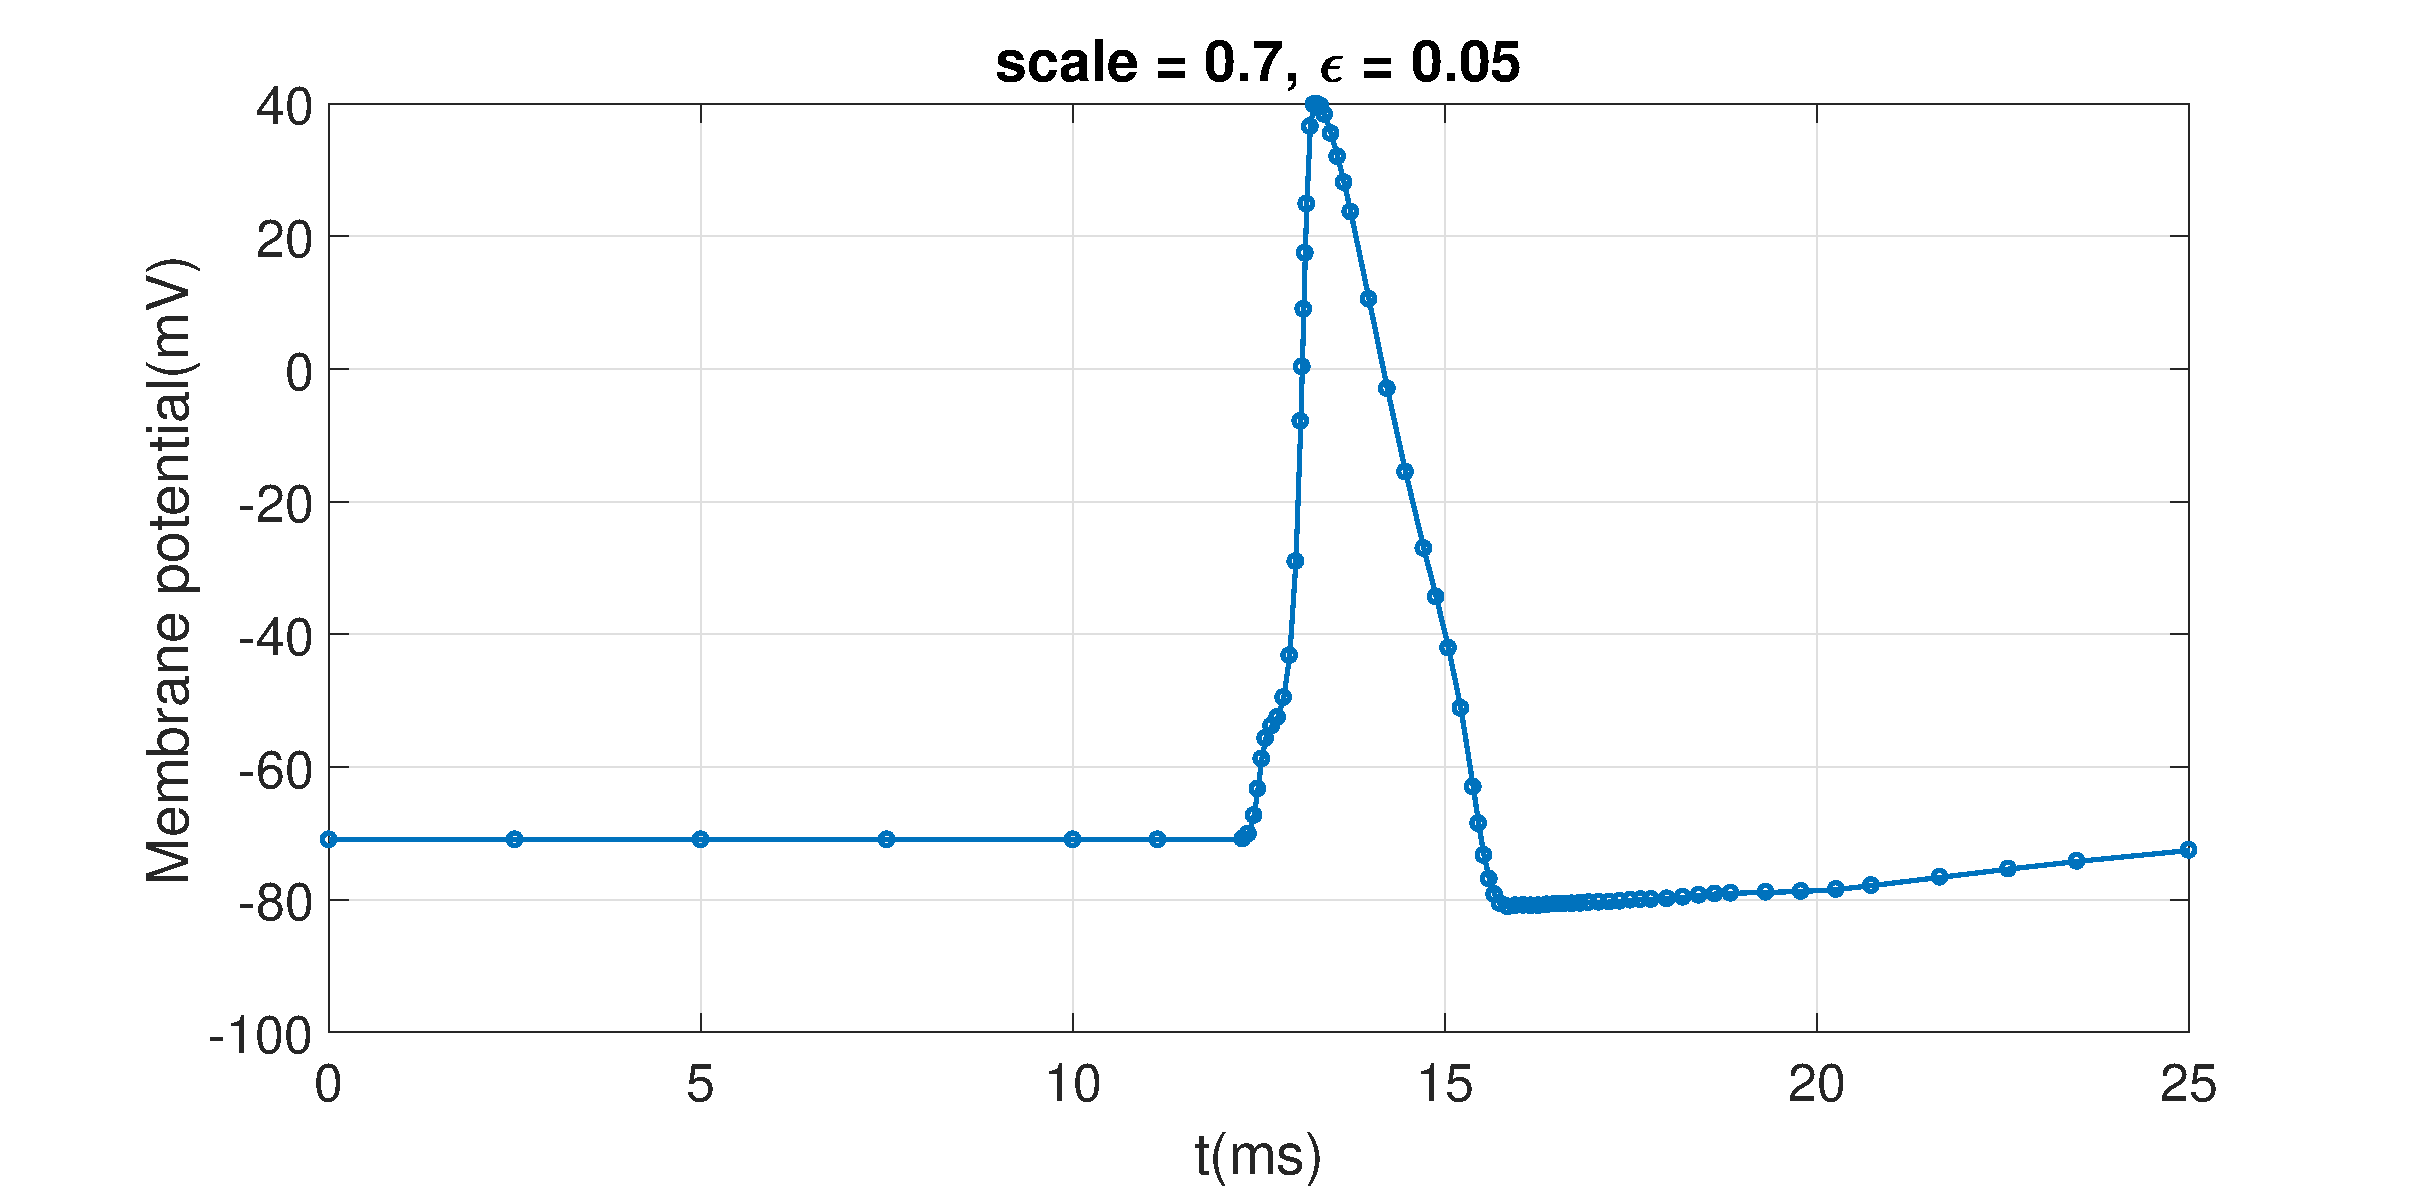
\includegraphics[width = 500pt]{705.eps}
	\end{figure}
	\begin{figure}[htbp]
		\centering
		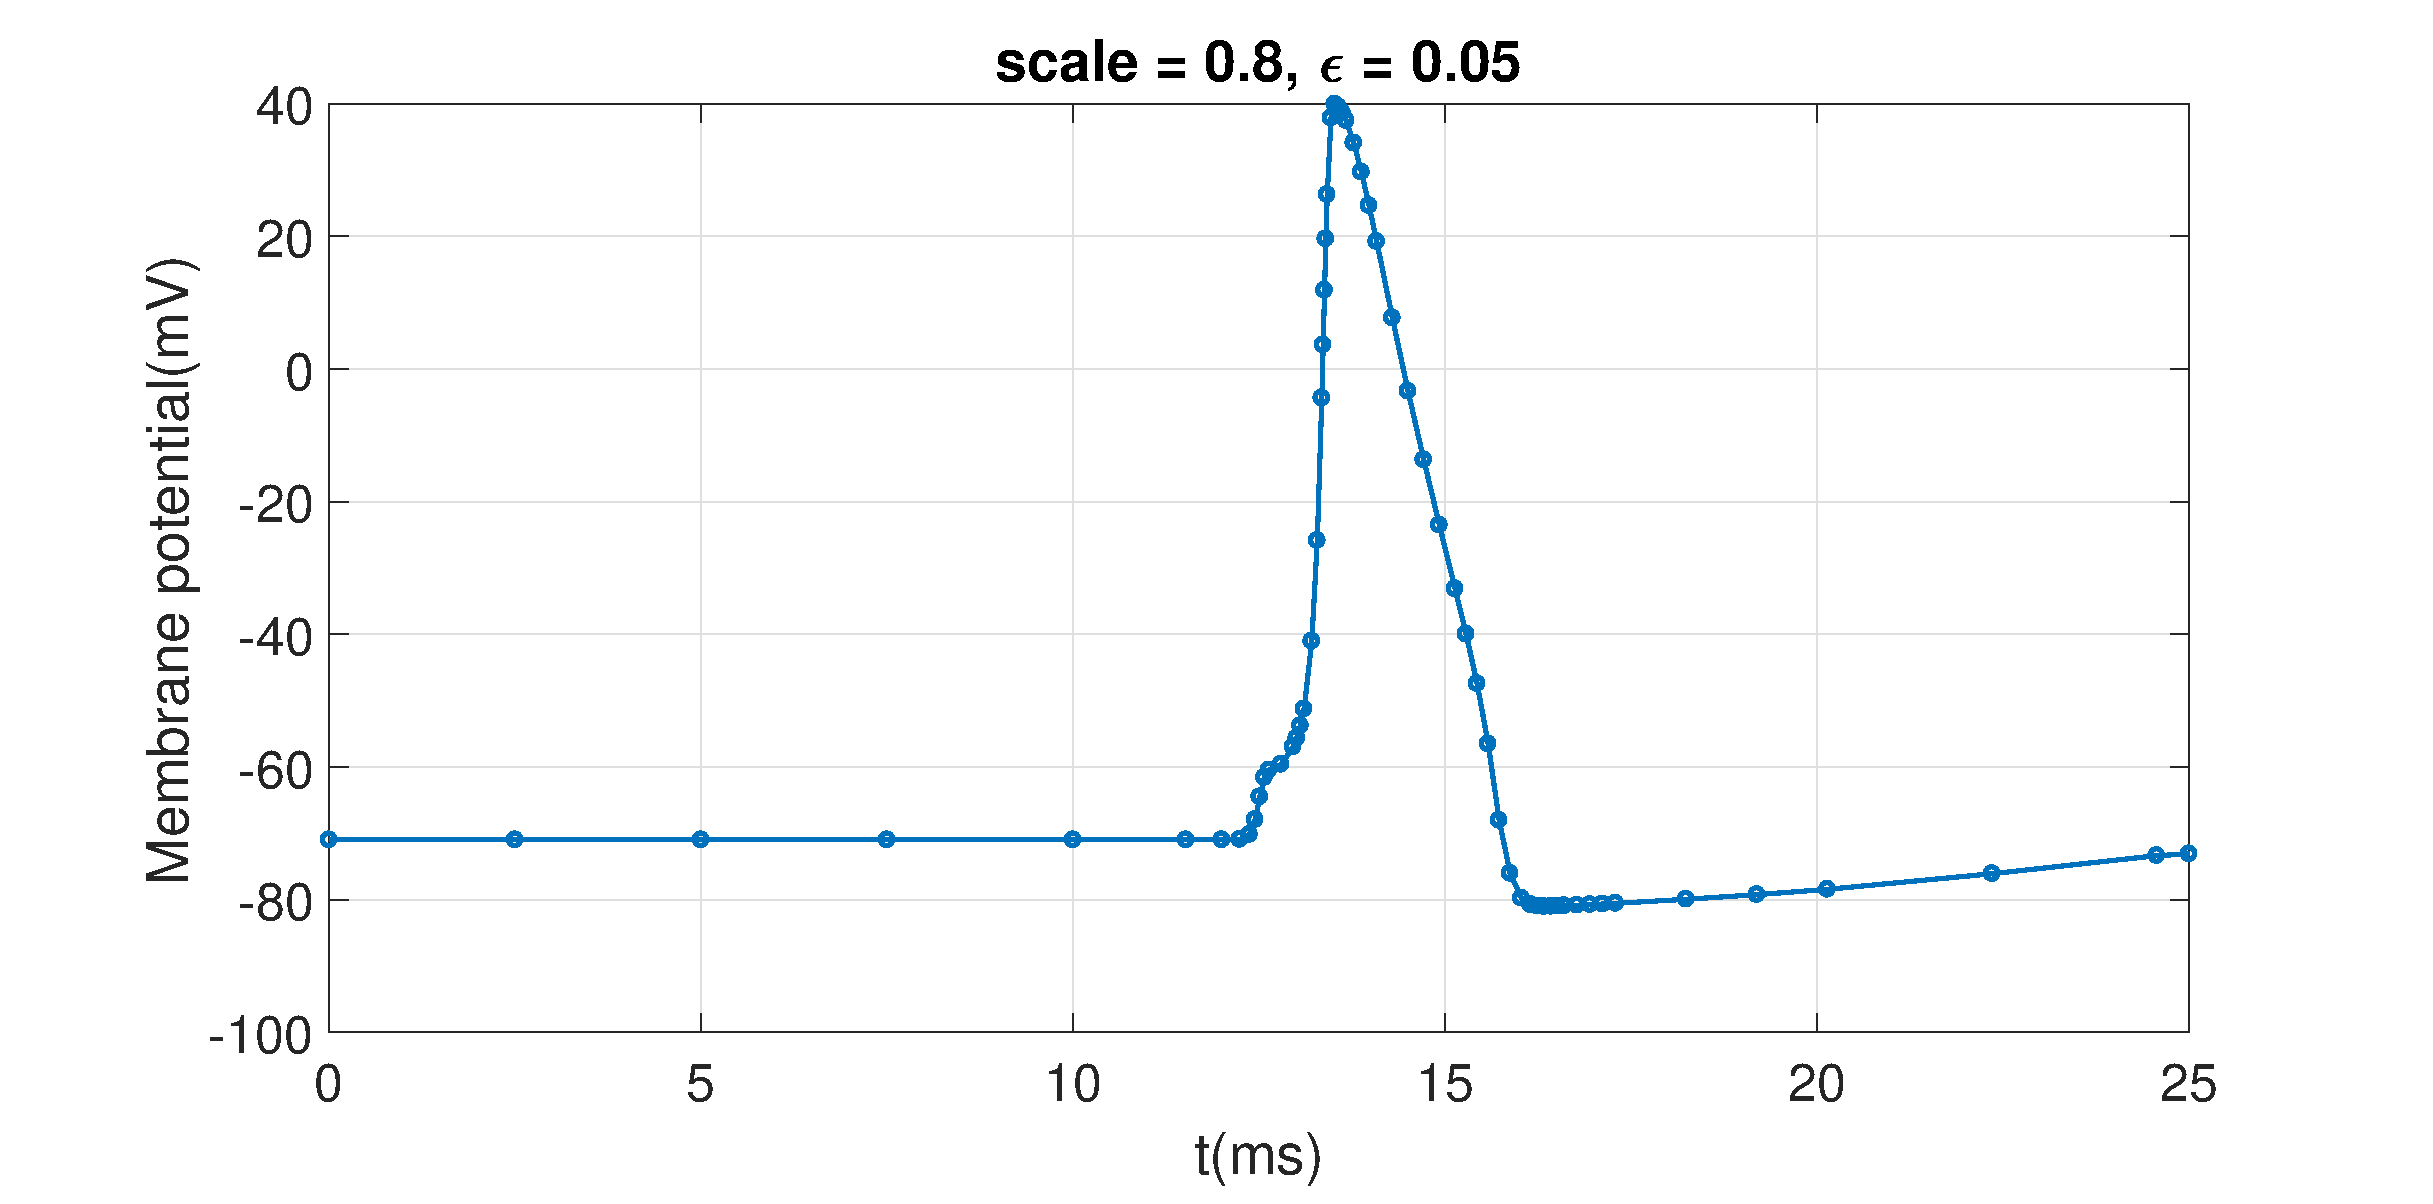
\includegraphics[width = 500pt]{805.eps}
	\end{figure}
	\end{CJK}
\end{document}